 \documentclass{article}

\usepackage{fancyhdr}
\usepackage{extramarks}
\usepackage{amsmath}
\usepackage{amsthm}
\usepackage{amsfonts}
\usepackage{amssymb}
\usepackage{xparse}
\usepackage{tikz}
\usepackage{graphicx}
\usepackage[plain]{algorithm}
\usepackage{algpseudocode}
\usepackage{listings}
\usepackage{hyperref}
\usepackage[per-mode = fraction]{siunitx}
\usepackage{calc}

\usetikzlibrary{automata,positioning}

\hypersetup{
    colorlinks=true,
    linkcolor=blue,
    filecolor=magenta,
    urlcolor=blue,
    }

\urlstyle{same}

%
% Basic Document Settings
%

\topmargin=-0.45in
\evensidemargin=0in
\oddsidemargin=0in
\textwidth=6.5in
\textheight=9.0in
\headsep=0.25in

\linespread{1.1}

\pagestyle{fancy}
\lhead{\hmwkAuthorName}
\chead{\hmwkClass\ (\hmwkClassInstructor,\ \hmwkClassTime): \hmwkTitle}
\rhead{\firstxmark}
\lfoot{\lastxmark}
\cfoot{\thepage}

\renewcommand\headrulewidth{0.4pt}
\renewcommand\footrulewidth{0.4pt}

\setlength\parindent{0pt}
\allowdisplaybreaks
%
% Title Page
%

\title{
	\vspace{2in}
	\textmd{\textbf{\hmwkClass:\ \hmwkTitle}}\\
	\normalsize\vspace{0.1in}\small{Due\ on\ \hmwkDueDate\ at \hmwkDueTime}\\
	\vspace{0.1in}\large{\textit{\hmwkClassInstructor,\ \hmwkClassTime}}
	\vspace{3in}
}
\author{\textbf{\hmwkAuthorName}}
\date{\hmwkCompletionDate}

%
% Create Problem Sections
%

\newcommand{\enterProblemHeader}[1]{
	\nobreak\extramarks{}{Problem #1 continued on next page\ldots}\nobreak{}
	\nobreak\extramarks{Problem #1 (continued)}{Problem #1 continued on next page\ldots}\nobreak{}
}

\newcommand{\exitProblemHeader}[1]{
	\nobreak\extramarks{Problem #1 (continued)}{Problem #1 continued on next page\ldots}\nobreak{}
	\nobreak\extramarks{Problem #1}{}\nobreak{}
}

%
% Homework Problem Environment
%
\NewDocumentEnvironment{hwkProblem}{m m s}{
	\section*{Problem #1: #2}
	\enterProblemHeader{#1}
	\setcounter{partCounter}{1}
}{
	\exitProblemHeader{#1}
	\IfBooleanF{#3} % if star, no new page
		{\newpage}
}

% Alias for the Solution section header
\newcommand{\hwkSol}{\vspace{\baselineskip / 2}\textbf{\Large Solution}\vspace{\baselineskip / 2}}

% Alias for the Solution Part subsection header
\newcounter{partCounter}
\newcommand{\hwkPart}{
	\vspace{\baselineskip / 2}
	\textbf{\large Part \Alph{partCounter}}
	\vspace{\baselineskip / 2}
	\stepcounter{partCounter}
}

%
% Various Helper Commands
%

% Such That
\newcommand{\st}{\text{s.t.}}

% Useful for algorithms
\newcommand{\alg}[1]{\textsc{\bfseries \footnotesize #1}}

% For derivatives
\newcommand{\deriv}[1]{\frac{\mathrm{d}}{\mathrm{d}x} (#1)}

% For partial derivatives
\newcommand{\pderiv}[2]{\frac{\partial}{\partial #1} (#2)}

% Integral dx
\newcommand{\dx}{\mathrm{d}x}
\newcommand{\dy}{\mathrm{d}y}

% Probability commands: Expectation, Variance, Covariance, Bias
\newcommand{\e}[1]{\mathrm{e}#1}
\newcommand{\E}{\mathrm{E}}
\newcommand{\Var}{\mathrm{Var}}
\newcommand{\Cov}{\mathrm{Cov}}
\newcommand{\Bias}{\mathrm{Bias}}

% Defining Units that are not in the SI base
\DeclareSIUnit\bar{bar}
\DeclareSIUnit\ft{ft}
\DeclareSIUnit\dollar{\$}
\DeclareSIUnit\cent{\text{\textcent}}
\DeclareSIUnit\c{\degreeCelsius}

% Code Listing config
\usepackage{xcolor}
\definecolor{codegreen}{rgb}{0,0.6,0}
\definecolor{codegray}{rgb}{0.5,0.5,0.5}
\definecolor{codepurple}{rgb}{0.58,0,0.82}
\definecolor{backcolour}{rgb}{0.95,0.95,0.92}
\lstdefinestyle{overleaf}{
	% backgroundcolor=\color{backcolour},
	commentstyle=\color{codegreen},
	keywordstyle=\color{magenta},
	numberstyle=\tiny\color{codegray},
	stringstyle=\color{codepurple},
	basicstyle=\ttfamily\footnotesize,
	breakatwhitespace=false,
	breaklines=true,
	captionpos=b,
	keepspaces=true,
	numbers=left,
	numbersep=5pt,
	showspaces=false,
	showstringspaces=false,
	showtabs=false,
	tabsize=4
}

\usepackage[latte]{catppuccinpalette}
\lstdefinestyle{catppuccin}{
	breaklines=true,
	keepspaces=true,
	numbers=left,
	numbersep=5pt,
	showspaces=false,
	showstringspaces=false,
	breakatwhitespace=true,
	tabsize=4,
	stringstyle = {\color{CtpGreen}},
	commentstyle={\color{CtpOverlay1}},
	basicstyle = {\small\color{CtpText}\ttfamily},
	keywordstyle = {\color{CtpMauve}},
	keywordstyle = [2]{\color{CtpBlue}},
	keywordstyle = [3]{\color{CtpYellow}},
	keywordstyle = [4]{\color{CtpLavender}},
	keywordstyle = [5]{\color{CtpPeach}},
	keywordstyle = [6]{\color{CtpTeal}}
}

\lstset{style=catppuccin}


%
% Homework Details
%   - Title
%   - Due date
%   - Due time
%   - Course
%   - Section/Time
%   - Instructor
%   - Author
%

\newcommand{\hmwkTitle}{Lab 04}
\newcommand{\hmwkDueDate}{October 27, 2024}
\newcommand{\hmwkDueTime}{11:59 PM}
\newcommand{\hmwkClass}{ENAE 380}
\newcommand{\hmwkClassTime}{0106}
\newcommand{\hmwkClassInstructor}{Dr. Mumu Xu}
\newcommand{\hmwkAuthorName}{\textbf{Vai Srivastava}}
\newcommand{\hmwkCompletionDate}{October 27, 2024}

\renewcommand{\solpart}[1]{\textbf{\large Part \arabic{partCounter}}\stepcounter{partCounter}}

\begin{document}

\maketitle
\pagebreak

\begin{hwkProblem}{6.1}{Inserting Noise}
	\solution

	\solpart

	\begin{lstlisting}[language=python]
		def noisy():
			f_main = 1000  # main frequency in Hz
			f_noise = 50   # noise frequency in Hz

			sample_rate = 48000  # samples per second
			duration = 10        # duration in seconds
			t = np.linspace(0, duration, duration * sample_rate, endpoint=False)  # time vector

			w_main = np.sin(2 * np.pi * f_main * t)  # main sine wave
			w_noise = np.sin(2 * np.pi * f_noise * t)  # noise sine wave
			w_combo = w_main + w_noise  # combined wave
			...
	\end{lstlisting}

	\newpage
	\solpart

	\begin{figure}[ht!]
	  \centering
	  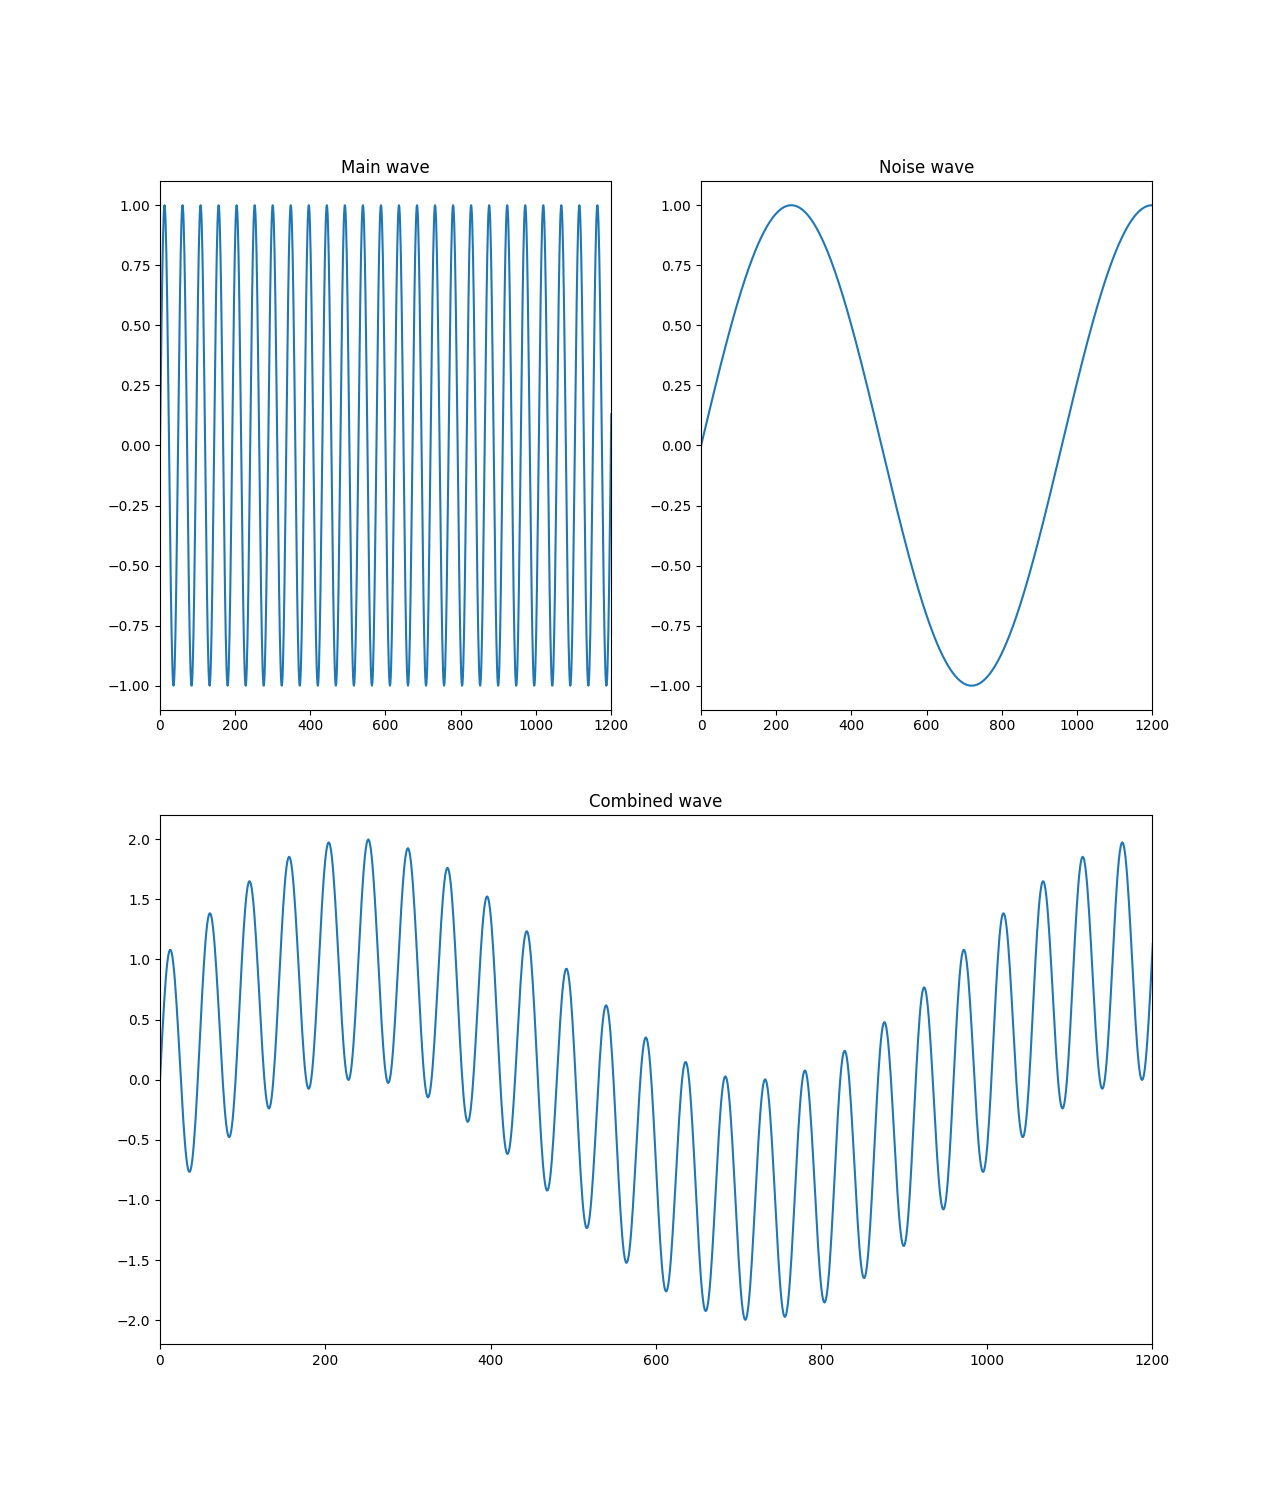
\includegraphics[width=0.85\textwidth]{./6.1.2.png}
	  \caption{Plots of Original, Noise, and Combined Waves}
	\end{figure}

	\newpage
	\solpart

	\begin{figure}[ht!]
	  \centering
	  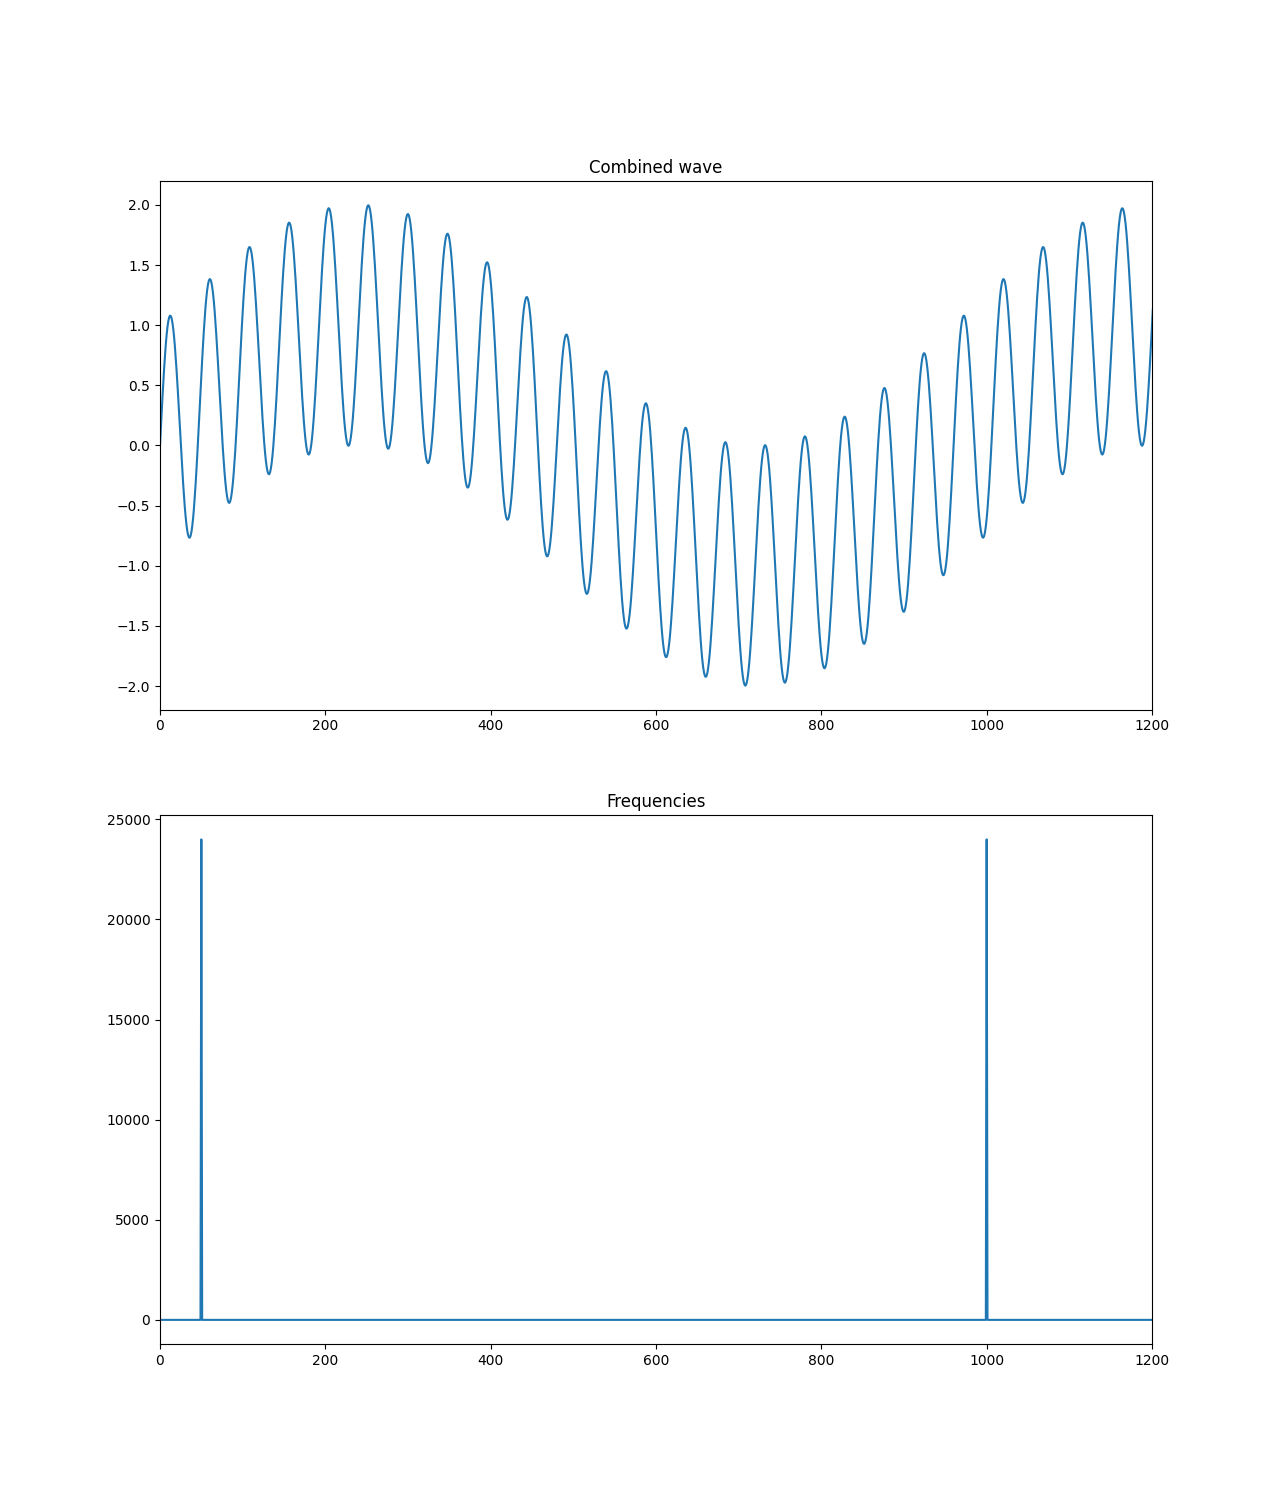
\includegraphics[width=0.85\textwidth]{./6.1.3.png}
	  \caption{Frequencies of Combined Wave}
	\end{figure}

	\newpage
	\solpart

	\begin{figure}[ht!]
	  \centering
	  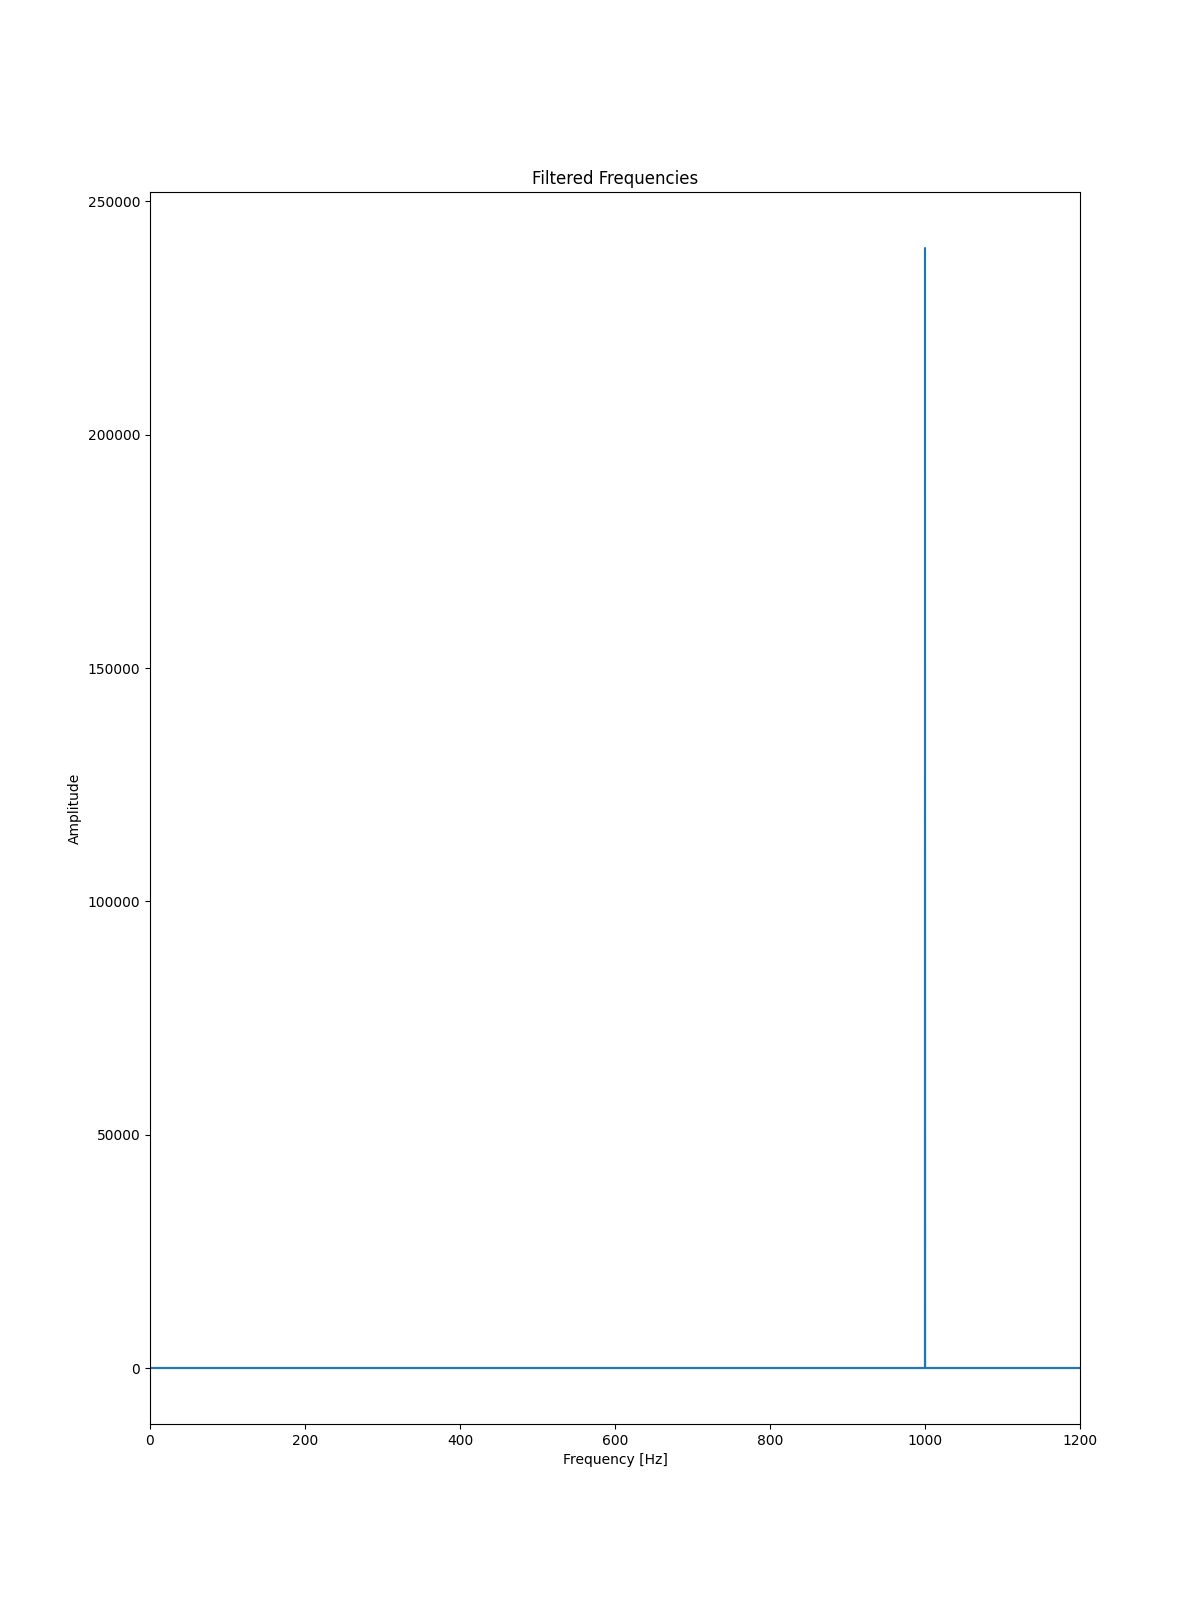
\includegraphics[width=0.85\textwidth]{./6.1.4.png}
	  \caption{Frequencies of Filtered Wave}
	\end{figure}

	\newpage
	\solpart

	\begin{figure}[ht!]
	  \centering
	  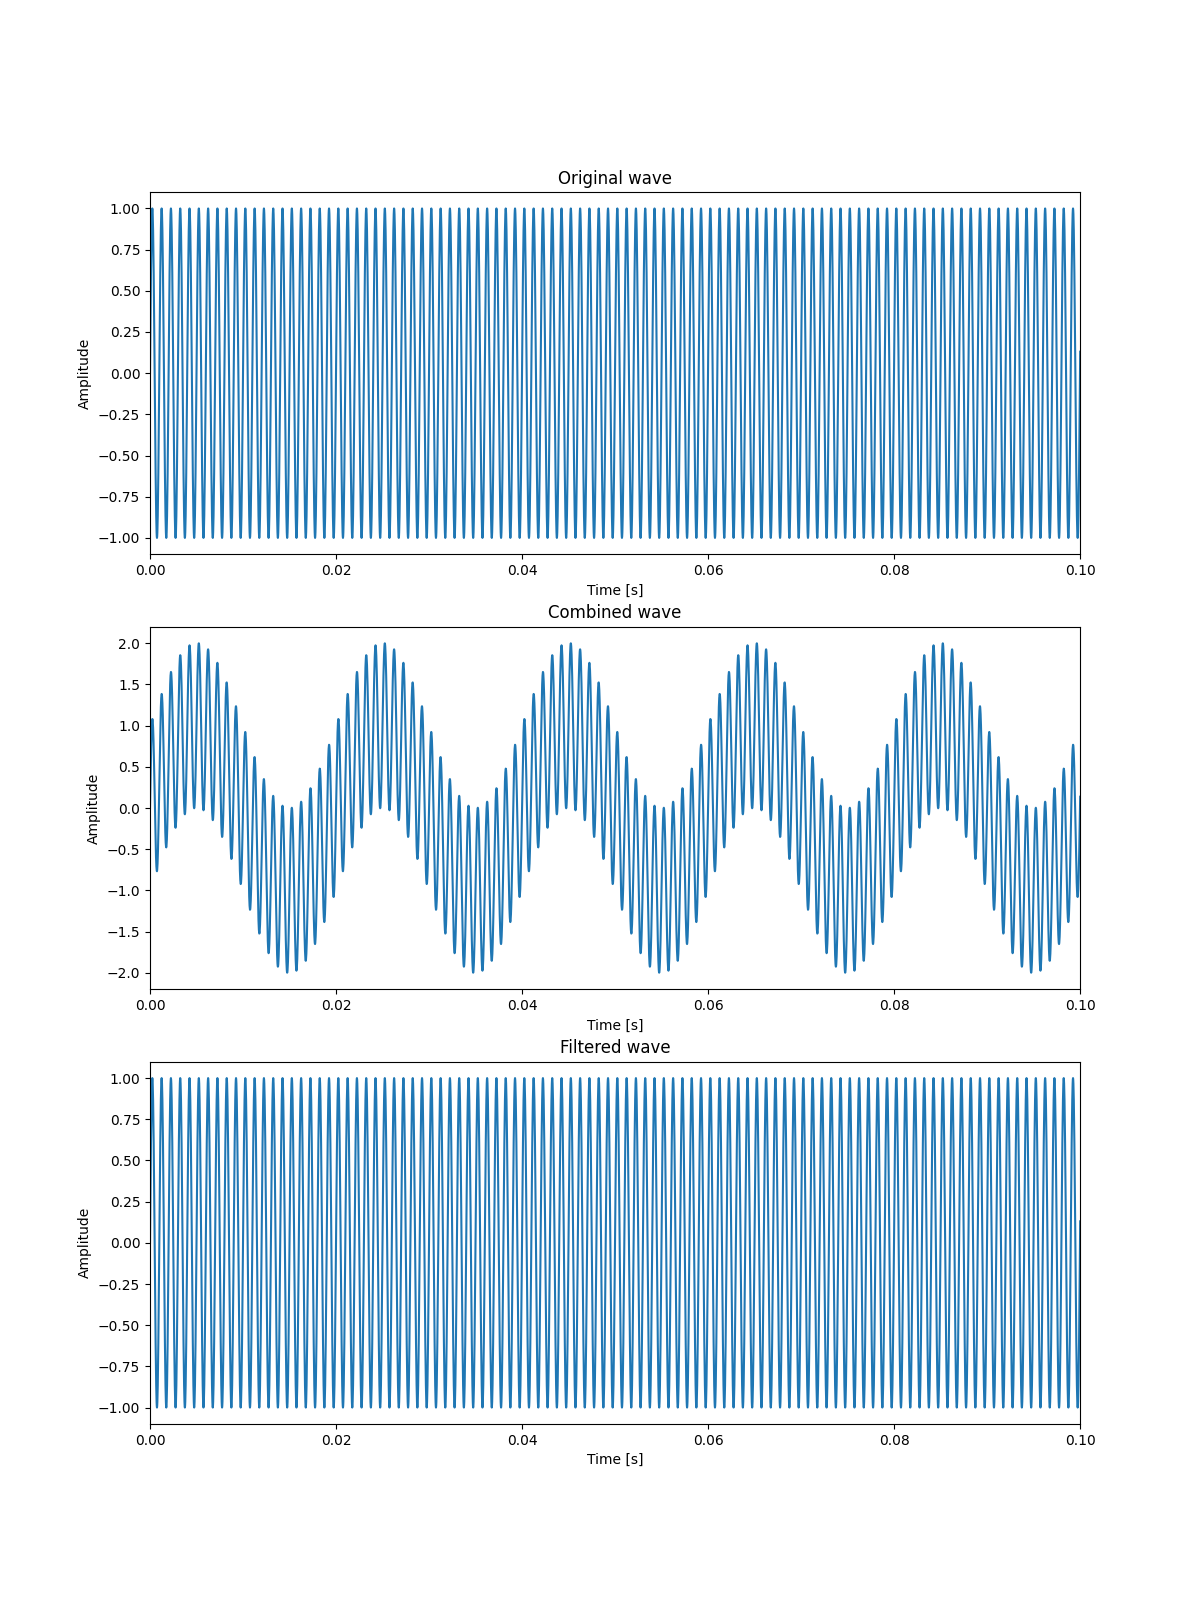
\includegraphics[width=0.85\textwidth]{./6.1.5.png}
	  \caption{Plots of Original, Combined, and Filtered Waves}
	\end{figure}

\end{hwkProblem}

\begin{hwkProblem}{6.2}{Pitch}
	\solution

	\solpart

	\begin{figure}[ht!]
	  \centering
	  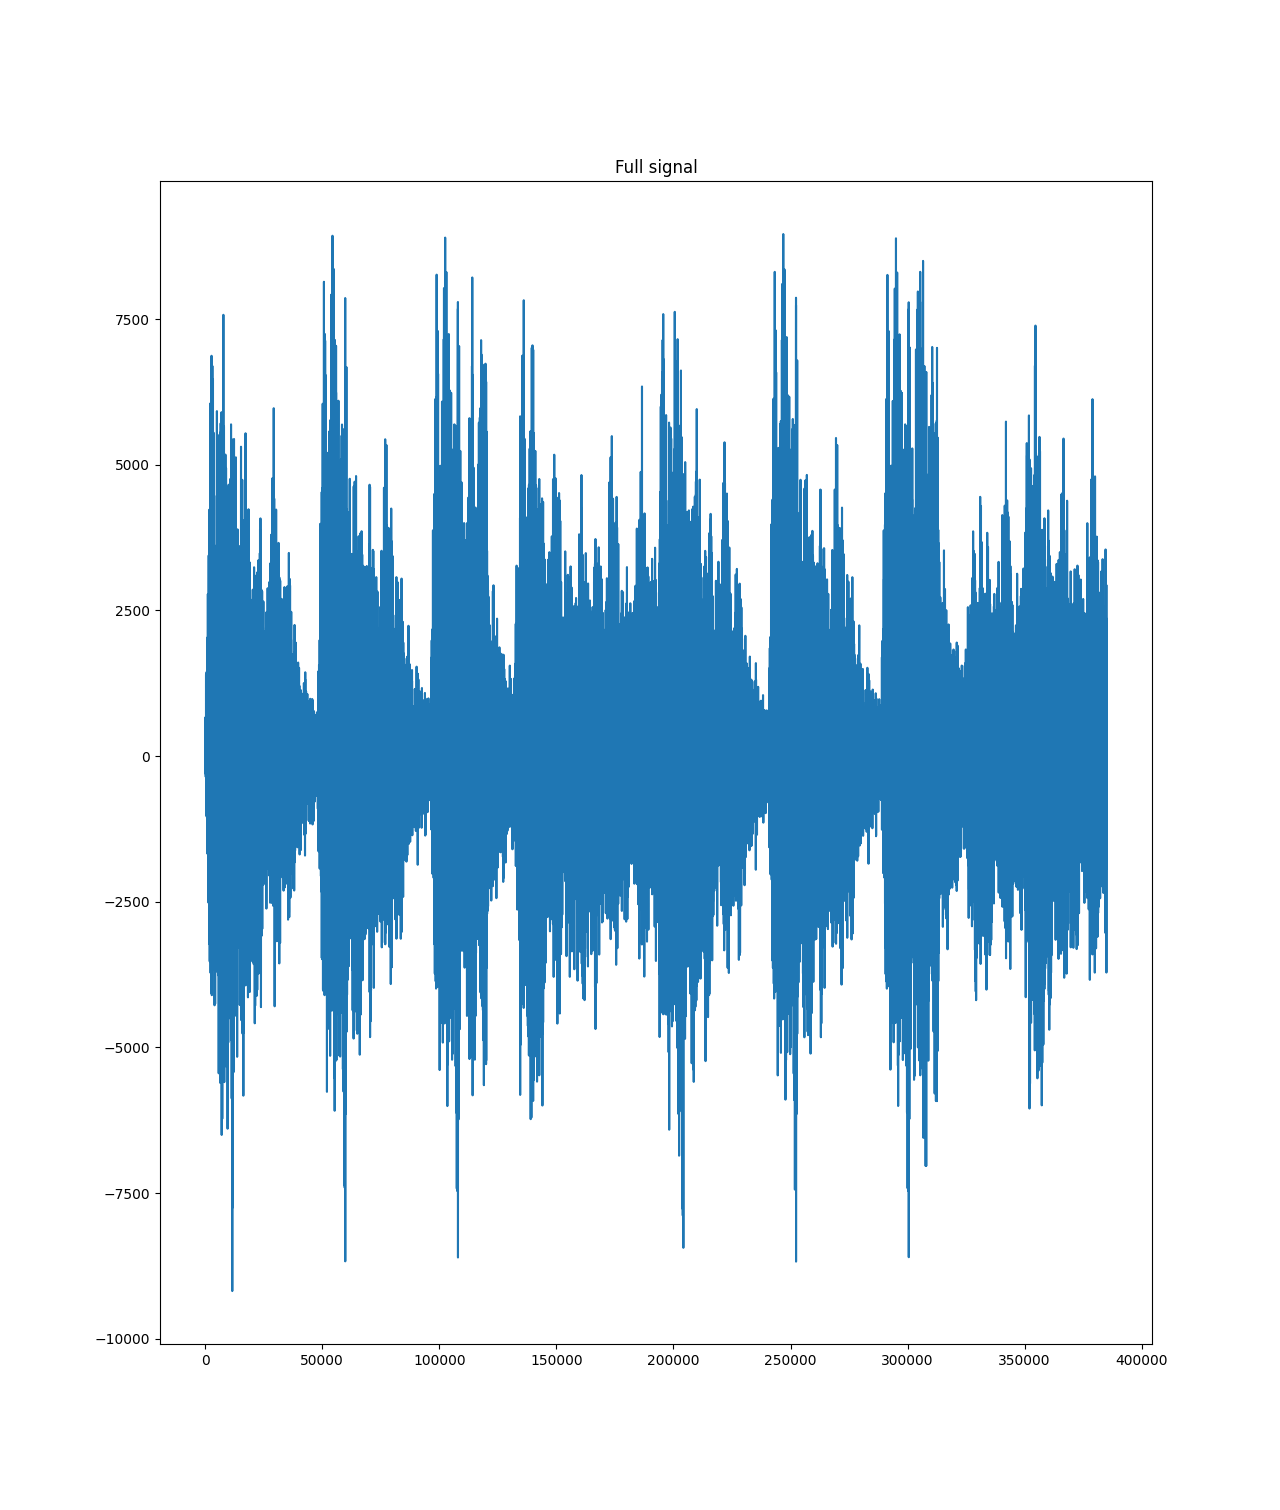
\includegraphics[width=0.85\textwidth]{./6.2.1.png}
	  \caption{Plot of \lstinline{trumpet.wav} Signal}
	\end{figure}

	\newpage
	\solpart

	\begin{figure}[ht!]
	  \centering
	  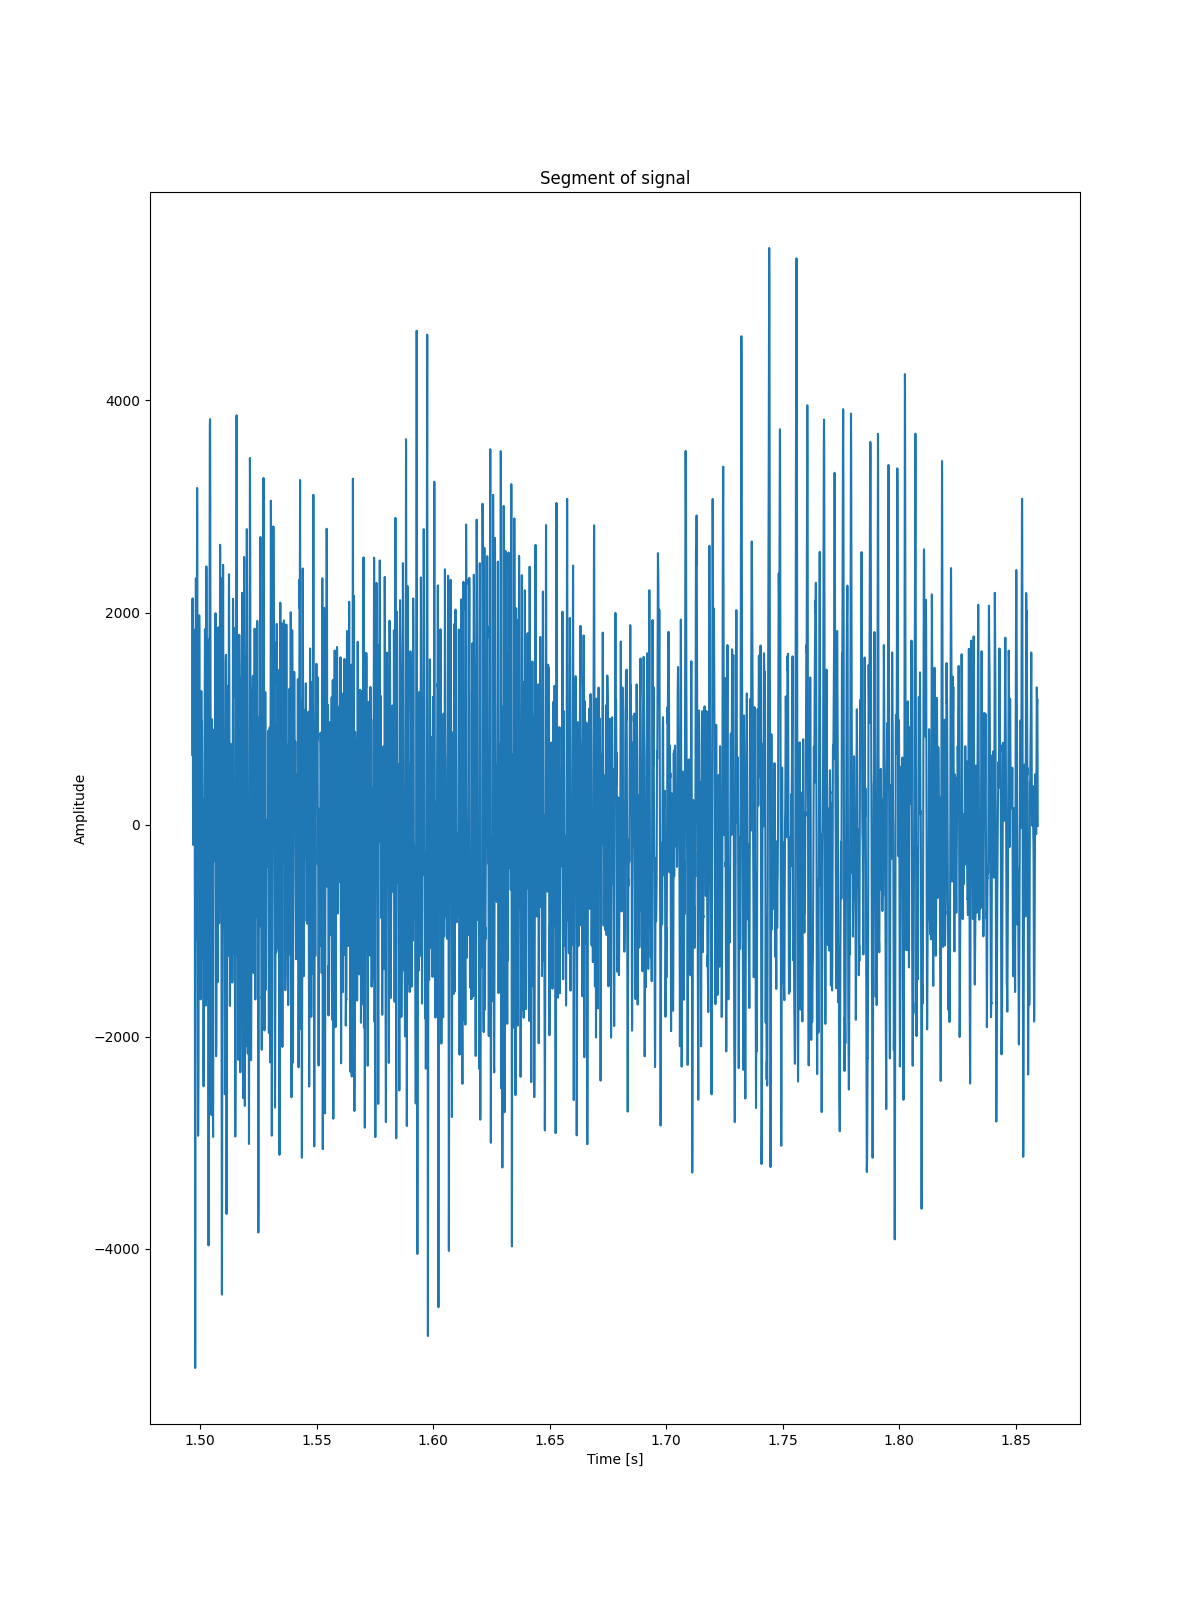
\includegraphics[width=0.85\textwidth]{./6.2.2.png}
	  \caption{Plot of Segment of Signal}
	\end{figure}

	\newpage
	\solpart

	\begin{figure}[ht!]
	  \centering
	  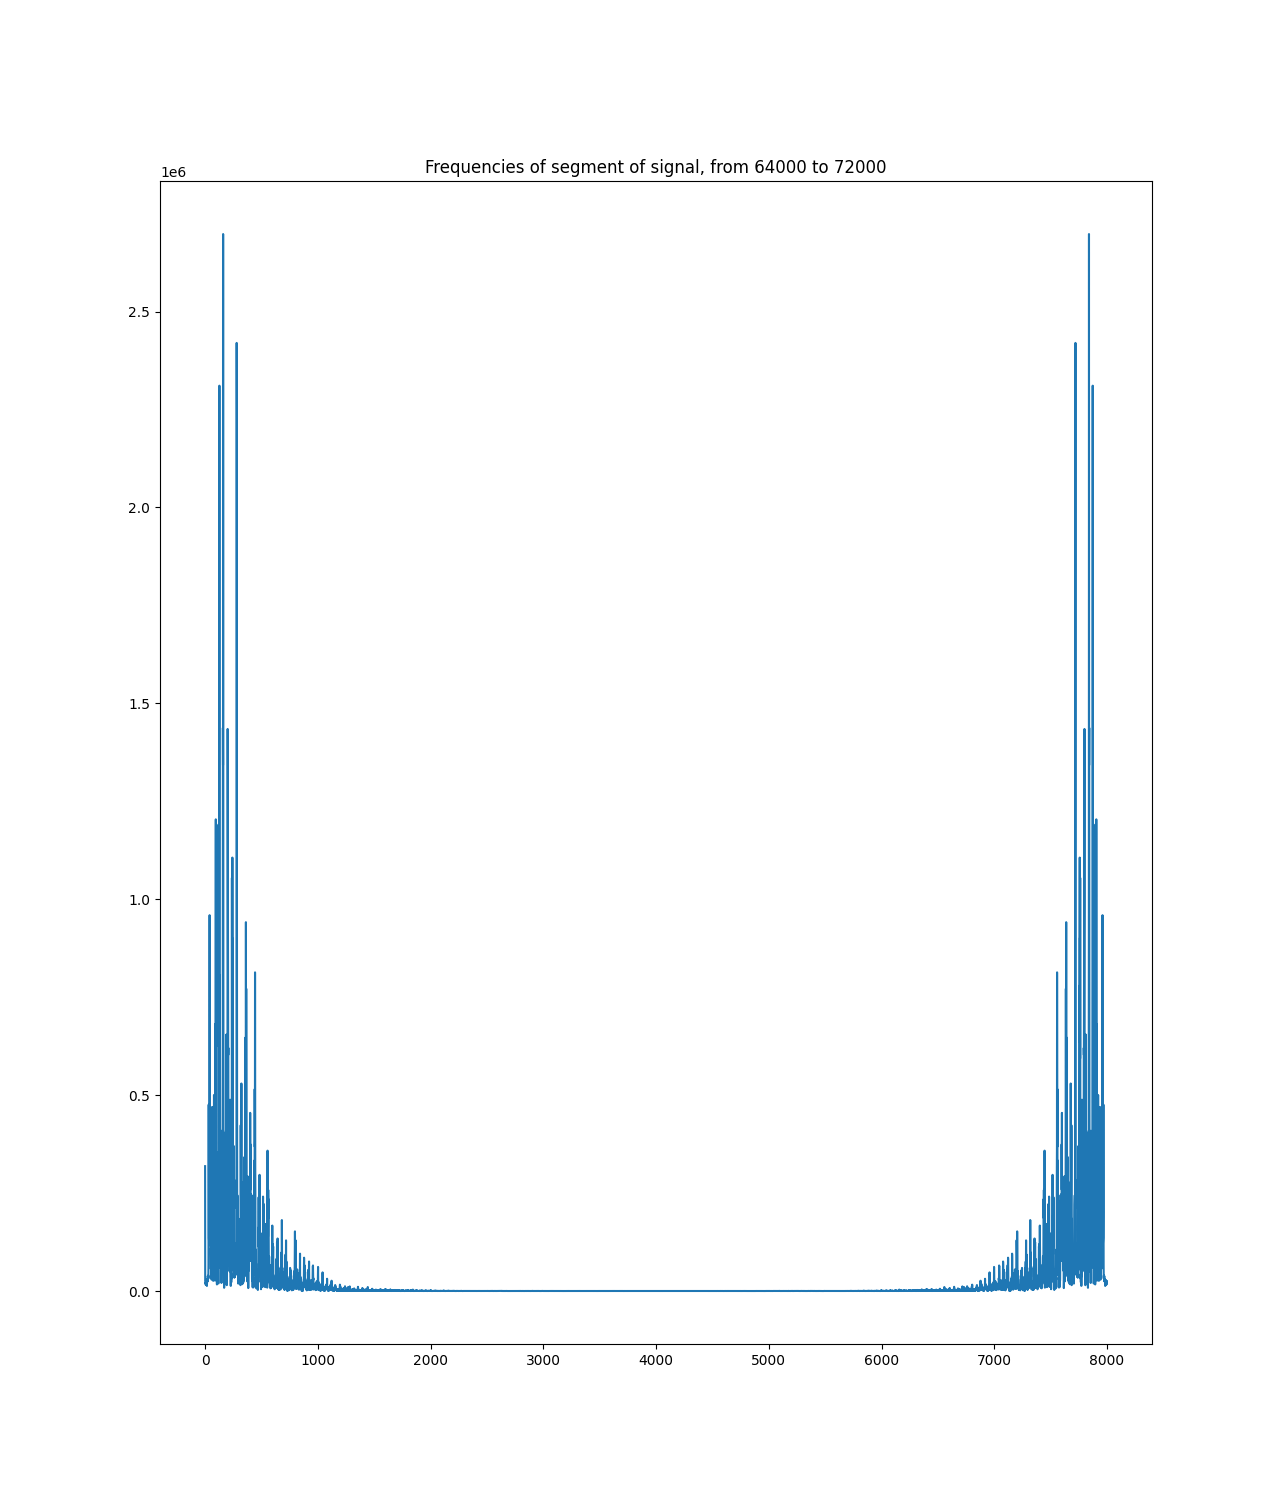
\includegraphics[width=0.85\textwidth]{./6.2.3.png}
	  \caption{Frequencies of Segment of Signal}
	\end{figure}

	\newpage
	\solpart

	\begin{lstlisting}[language=python]
		def pitch():
			...
			positive_freqs = fftf_seg[: fftf_seg.size // 2]
			positive_fft = fftw_seg[: fftw_seg.size // 2]

			three_highest_locs = np.argpartition(np.abs(positive_fft), -3)[-3:]

			three_highest_freqs = positive_freqs[three_highest_locs]
			three_highest_vals = positive_fft[three_highest_locs]

			print("Corresponding frequencies [Hz]:", three_highest_freqs)
			print("Amplitudes of the three highest frequencies:", np.abs(three_highest_vals))
			...
	\end{lstlisting}

	\begin{lstlisting}[language=python]
		Corresponding frequencies [Hz]: [104.7375  107.49375 124.03125]
		Amplitudes of the three highest frequencies: [ 8628544.04894822  9302906.62716424 10746634.73638791]
	\end{lstlisting}

	\newpage
	\solpart

	\begin{lstlisting}[language=python]
		def pitch():
			...
			# Zero out the three highest frequencies
			fftw_seg[three_highest_locs] = 0
			fftw_seg[-three_highest_locs] = 0
			...
	\end{lstlisting}

	\newpage
	\solpart

	\begin{figure}[ht!]
	  \centering
	  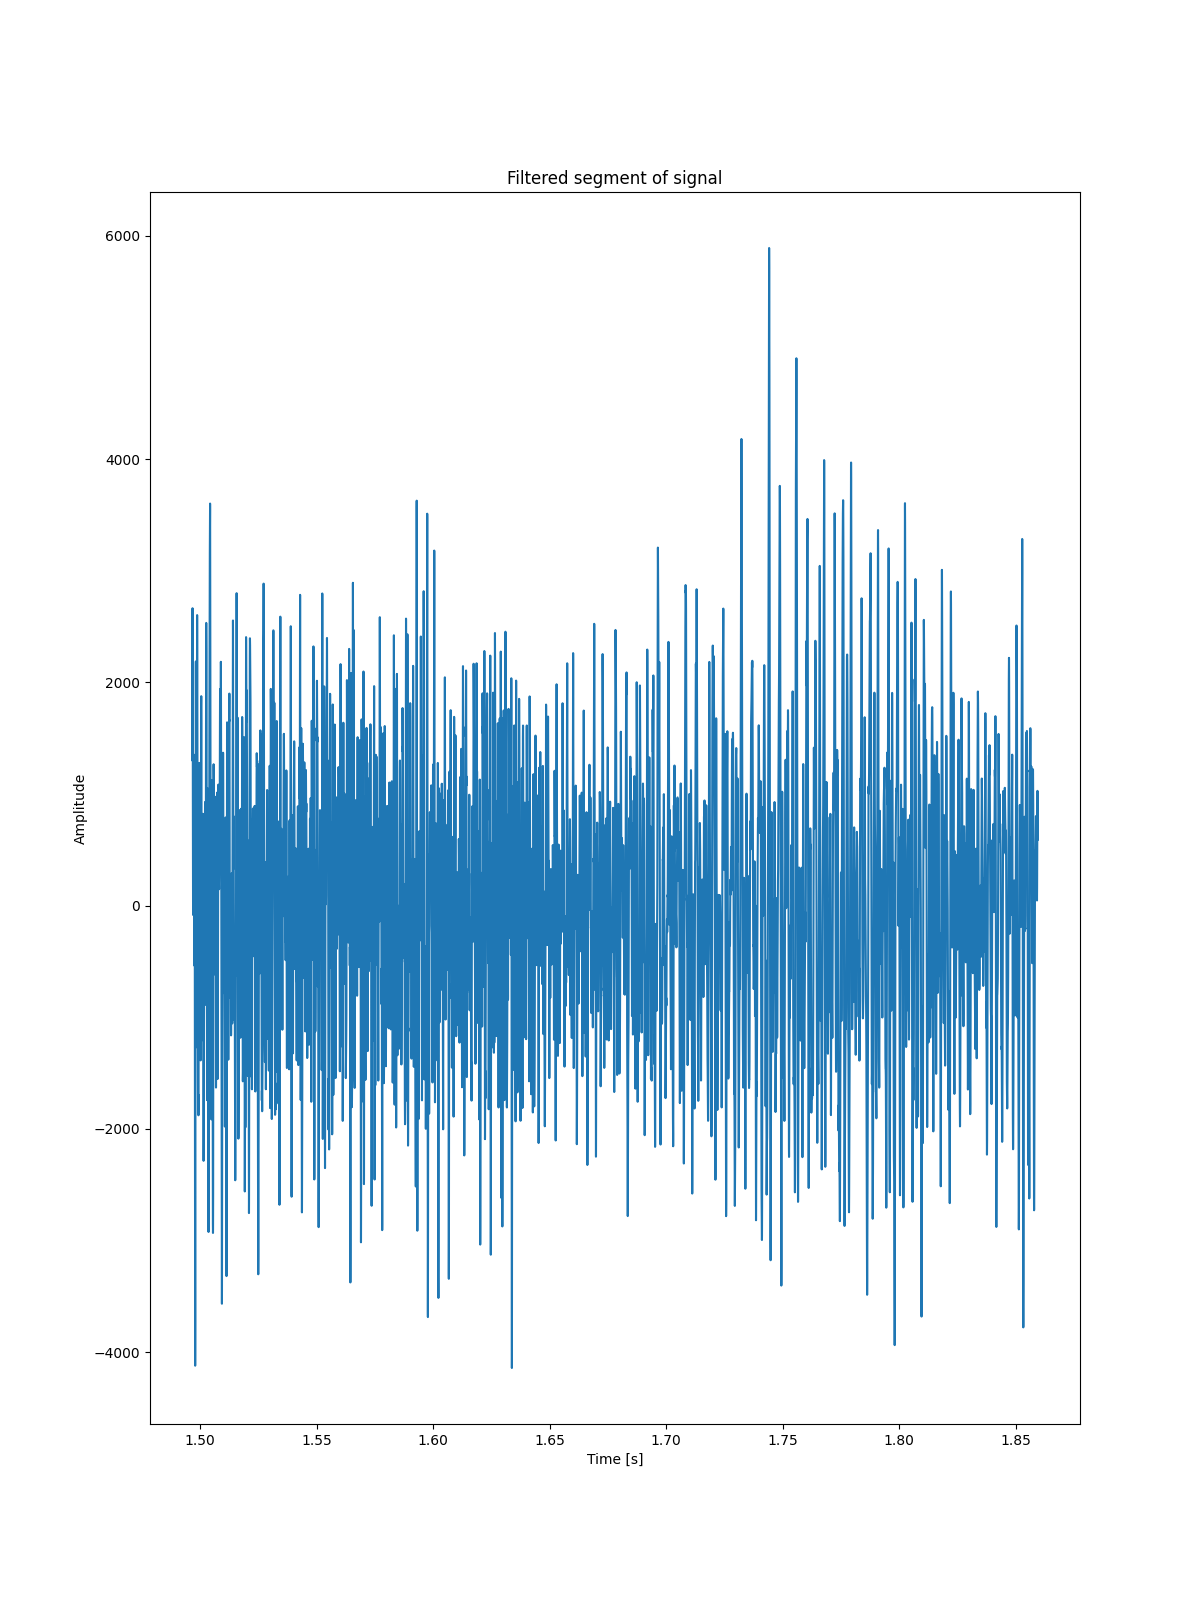
\includegraphics[width=0.85\textwidth]{./6.2.6.png}
	  \caption{Plot of Filtered Segment of Signal}
	\end{figure}

	\newpage
	\solpart

	\begin{lstlisting}[language=python]
		def pitch():
			...
			# Normalize and save the filtered segment as a wav file
			w_filtered_norm = (w_filtered / np.max(np.abs(w_filtered)) * 32767).astype(np.int16)

			wave.write("segment_filter.wav", sample_rate, w_filtered_norm)
			...
	\end{lstlisting}

\end{hwkProblem}

\begin{hwkProblem}{6.3}{Mixing Signals}
	\solution

	\begin{figure}[ht!]
	  \centering
	  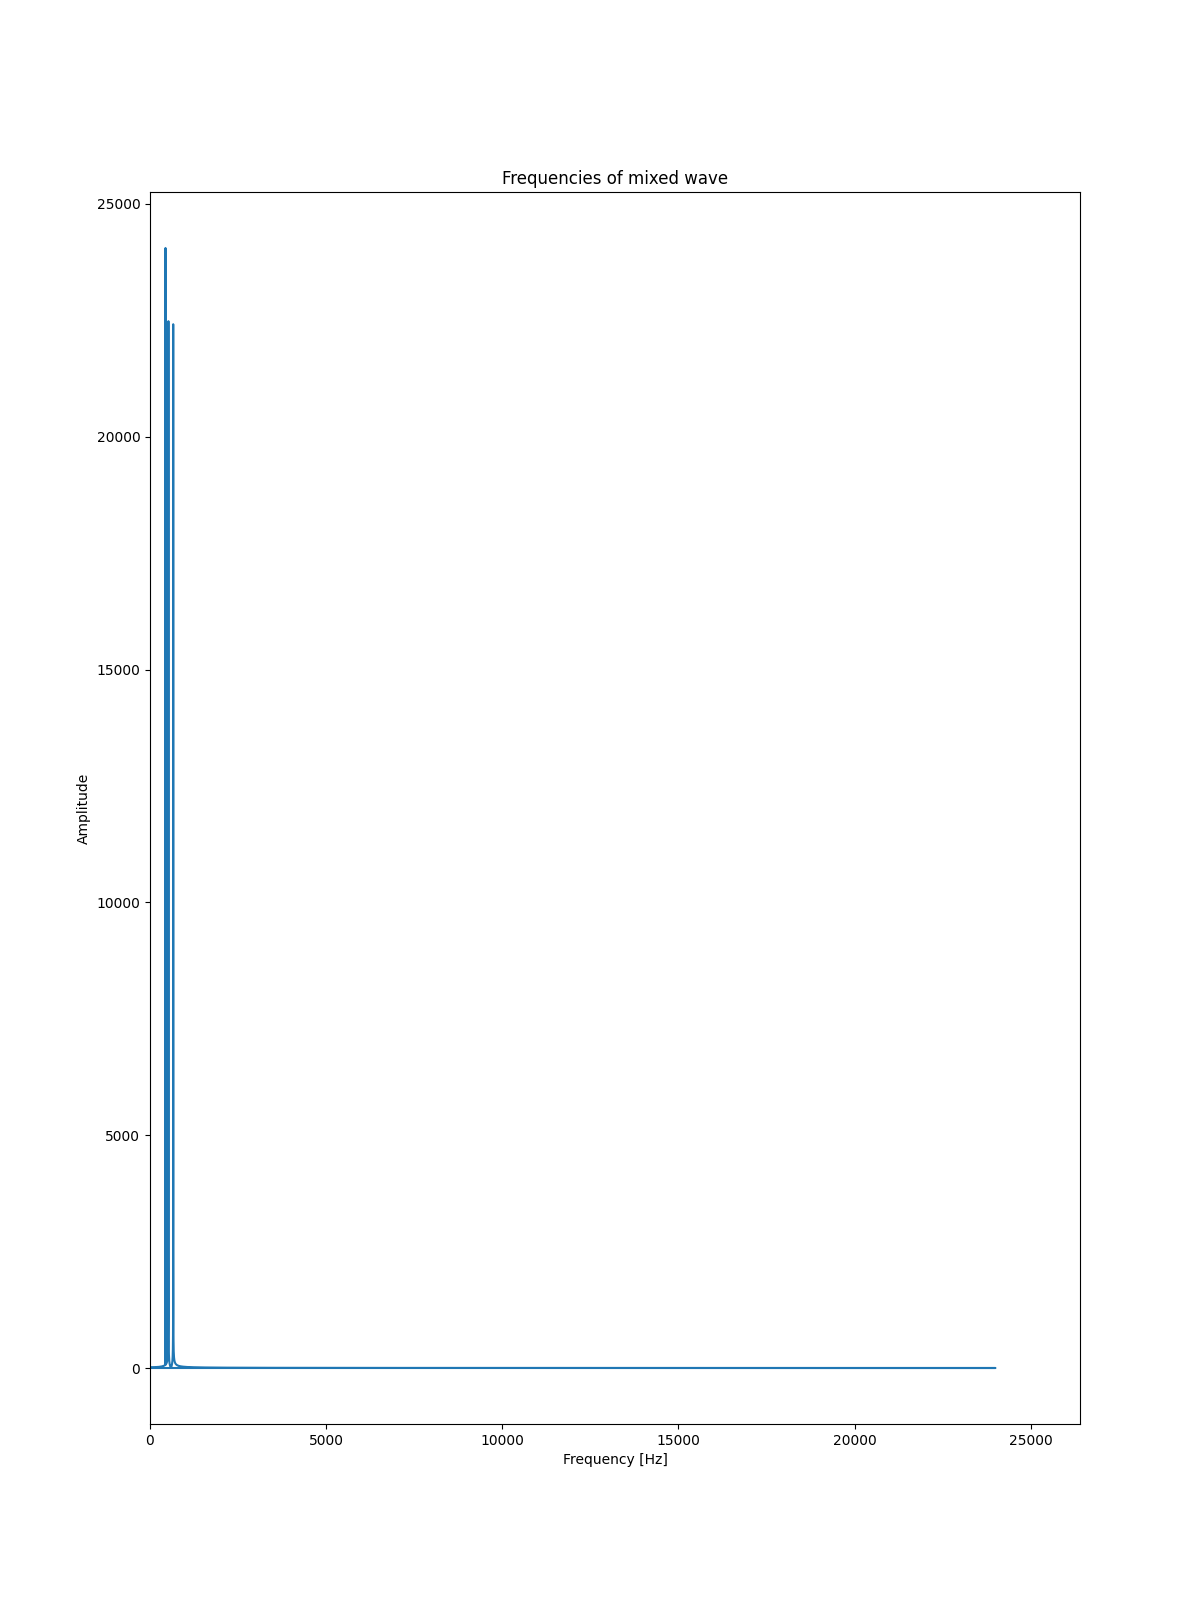
\includegraphics[width=0.75\textwidth]{./6.3.png}
	  \caption{Frequencies of Mixed Wave}
	\end{figure}

	When adding frequencies that are not multiples of the fundamental frequency, you get a tone that is out of phase with the original signal. This can be tonally harsh, or it can be tonally good. How it sounds is really up to the listener, which is why music is subjective and can take on many forms.
	
\end{hwkProblem}

\begin{hwkProblem}{6.4}{Stretch}
	\solution

	\begin{lstlisting}[language=python]
		def stretch(input, output, factor):
			"""
			Stretch or compress a wav file by changing its sample rate.

			Parameters:
			- input: path to input wav file
			- output: path to output wav file
			- factor: stretching factor (e.g., 0.75 to compress, 1.25 to stretch)
			"""
			sample_rate, w_input = wave.read(input)
			wave.write(output, int(sample_rate * factor), w_input)
	\end{lstlisting}
\end{hwkProblem}

\begin{hwkProblem}{6.5}{Sampling}
	\solution

	\solpart

	\begin{figure}[ht!]
	  \centering
	  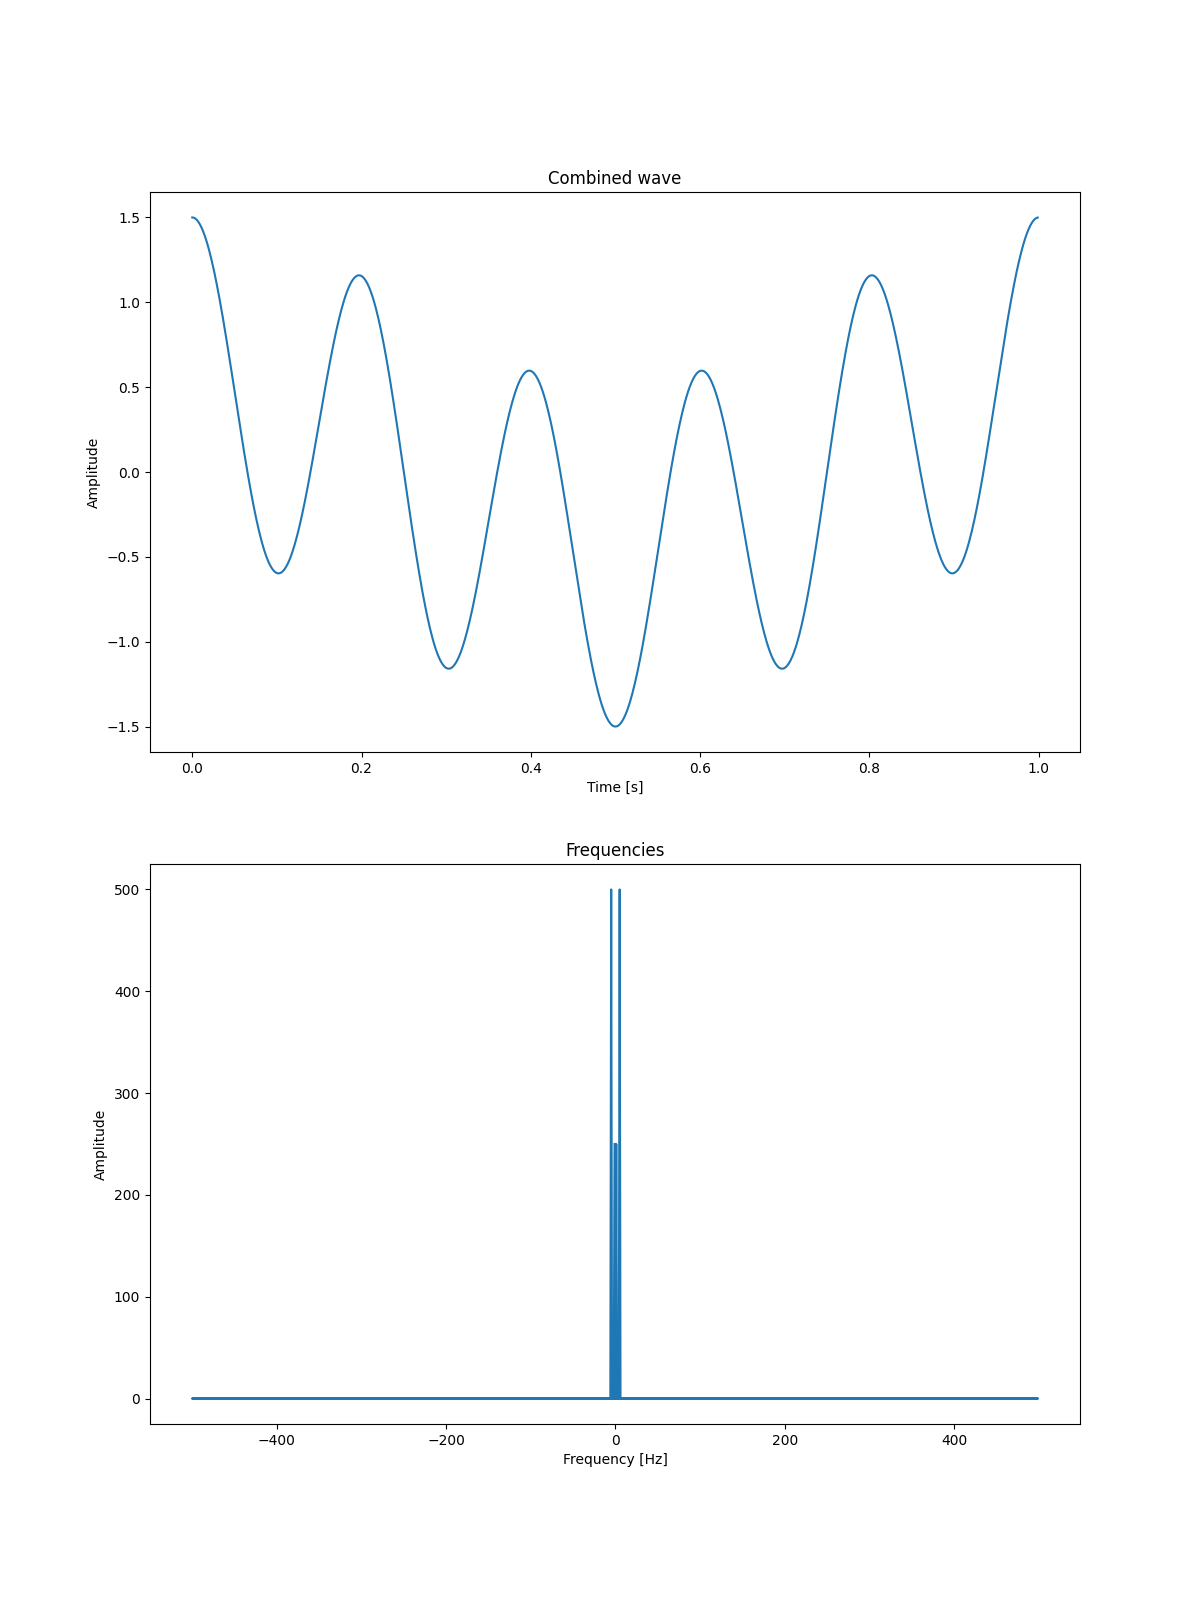
\includegraphics[width=0.75\textwidth]{./6.5.1.png}
	  \caption{Plot of Provided Wave and Frequencies}
	\end{figure}

	\newpage
	\solpart

	\begin{lstlisting}[language=python]
		def sampling():
			...
			# Subsample the signal
			F = 125  # new sample rate in Hz
			subsample_factor = int(sample_rate / F)

			w_sub = w_og[::subsample_factor]  # subsampled wave
			t_sub = t_og[::subsample_factor]  # subsampled time vector
			...
	\end{lstlisting}

	\newpage
	\solpart

	\begin{figure}[ht!]
	  \centering
	  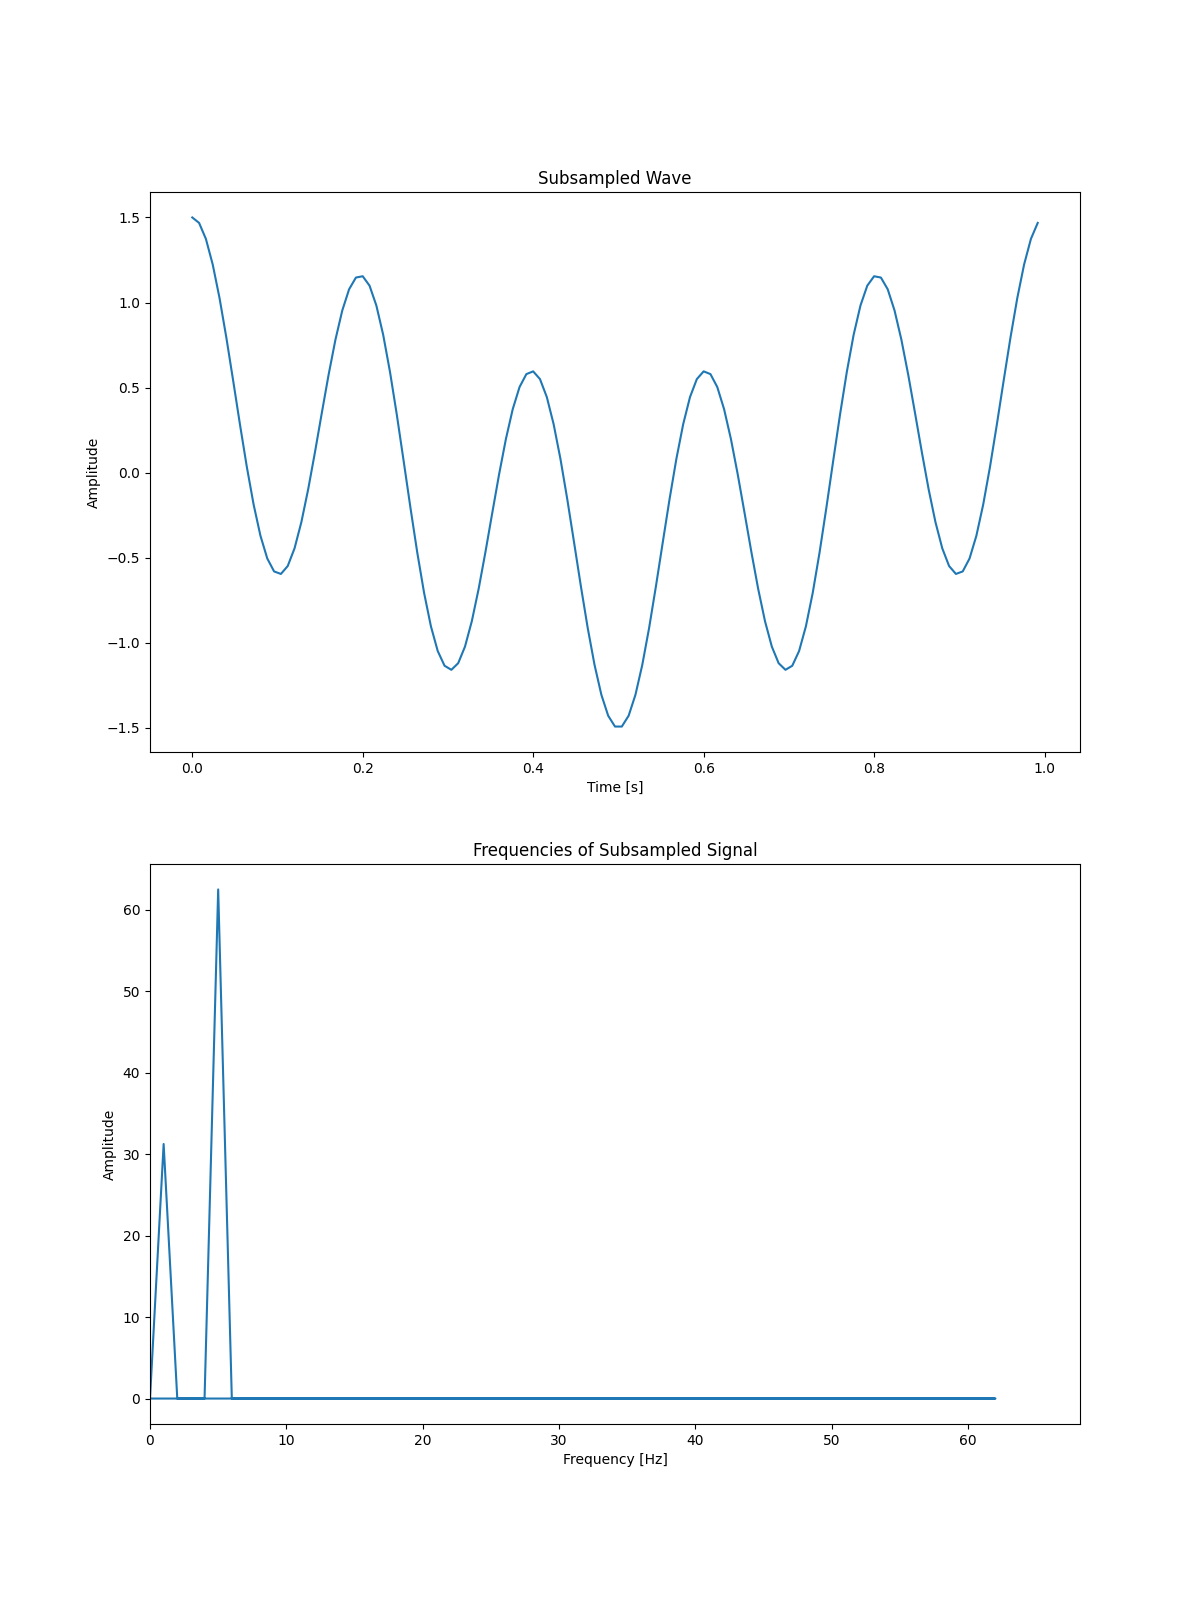
\includegraphics[width=0.85\textwidth]{./6.5.3.png}
	  \caption{Plot of Sub-Sampled Wave and Frequencies}
	\end{figure}

	\newpage
	\solpart
	\linebreak
	
	The signal starts degrading at all frequencies below the half the sampling rate (i.e. \( \forall f \in f := \frac{1}{F}, F < B, B := \frac{f_s}{2} \)). This is due to the bandwith of our signal being limited by the Nyquist sampling criterion\footnote{Ref: \href{https://doi.org/10.1109/JRPROC.1949.232969}{DOI: 10.1109/JRPROC.1949.232969}}, which defines the above mathematical model, and states that any reconstruction of a signal that was analyzed at such framerate will only have a perfect reconstruction when \( B \), the bandlimit, is less than half of the original sampling rate (i.e. \( 2B < f_s \)). In regular terms, this means that we are sampling at intervals that are too small to contain a complete spectrum of information, and thus, our reconstruction is negatively impacted.
	
\end{hwkProblem}

\end{document}
